% Hazi Feladat / Meresi jegyzokony sablon BME MIT
% Keszult: 2012.13.17
% Leiras: Ebbe a fajlba kerul a lenyegi resz, a szoveg. A legfelsobb szintu felsorolas a section (chapter nem hasznalatos).

\section{A mérés bemutatása}


\section{Otthoni feladat 1}
\subsection{Leírás}
A laborsegédlet és az egyéb segédanyagok maradéktalan elolvasását és megértését követően
töltse le a labor weblapjáról ( http://www.mit.bme.hu/oktatas/targyak/vimim223/feladat/5-Szavazas-es-aukcio ) a
labor forráskódjait, és bontsa ki a forráskódokat a  msclab01 könyvtárba. Ezt
követően indítson el Eclipse alól egy JADE platform-ot, majd legalább három
msclab01.votingauction\_lab.VoterAgent.VoterAgent szavazó ágenst (pl.  va0 ,
va1 , és  va2 néven) a voting01.cfg szavazási
konfigurációnak megfelelő – akár egyező, akár különböző – jelöltekkel, illetve egy
msclab01.votingauction\_lab.VotingMechanismAgent.VotingMechanismAgent
szavazásvezérlő ágenst (pl.  vma néven) az előbb említett konfigurációval.
\begin{enumerate}
	\item Figyelje meg és értelmezze a működést.
	\item Kövesse nyomon Sniffer ágenssel az ágensek közti üzenetcserét.
	\item Mit tapasztal?
	\item Más-más szavazó ágens paraméterek megadása hatására hogy viselkedik a rendszer?
	\item Milyen szabályok szerint zajlik a szavazás?
	\item Mi az előnye, és mi a hátulütője ennek a fajtájú szavazásnak?
	\item A lefutás során/után milyen adatok jöttek létre a log
	könyvtárban?
\end{enumerate}
\subsection{Megoldás}
Futattam az ágenseket a következő run config-ot használva:
\begin{lstlisting}[caption=Szavazás run config, frame=single,float=!ht]
-container  -port  1099  -host  localhost
AAAAAA:msclab01.votingauction\_lab.VoterAgent.VoterAgent(mathias)
BBBBBB:msclab01.votingauction\_lab.VoterAgent.VoterAgent(mandela)
CCCCCC:msclab01.votingauction\_lab.VoterAgent.VoterAgent(mandela)
DDDDDD:msclab01.votingauction\_lab.VoterAgent.VoterAgent(valakimas) vma:msclab01.votingauction_lab.VotingMechanismAgent.VotingMechanismAgent(cfg\backslash voting01.cfg)
\end{lstlisting}
\begin{figure}[!h]
\begin{center}
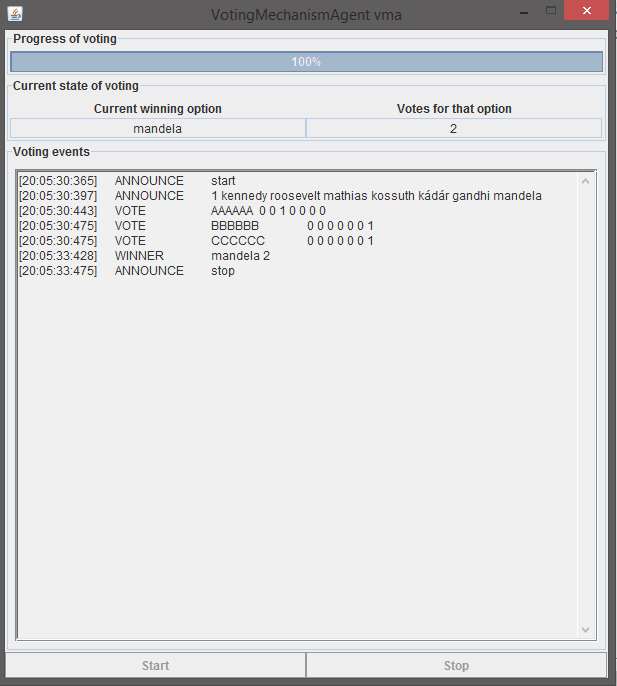
\includegraphics[height=7cm]{figures/ofel1a1.png}
\caption{A szavazás eredménye}
\end{center}
\end{figure}
\begin{figure}[!h]
\begin{center}
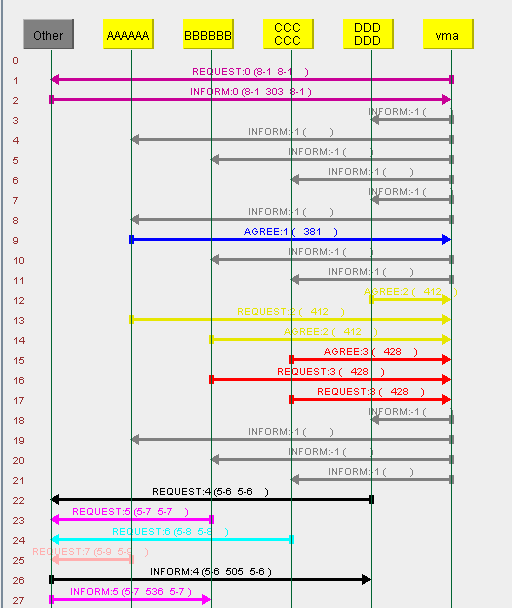
\includegraphics[height=7cm]{figures/ofel1a2.png}
\caption{Az ágensek közötti komunikáció}
\end{center}
\end{figure}
\begin{lstlisting}[caption=A log.txt tartalma, frame=single,float=!ht]
[20:16:23:533]	ANNOUNCE	start
[20:16:23:549]	ANNOUNCE	1 kennedy roosevelt mathias kossuth kádár gandhi mandela
[20:16:23:565]	VOTE		BBBBBB	0 0 0 0 0 0 1
[20:16:23:565]	VOTE		AAAAAA	0 0 1 0 0 0 0
[20:16:23:580]	VOTE		CCCCCC	0 0 0 0 0 0 1
[20:16:26:596]	WINNER	mandela 2
[20:16:26:596]	ANNOUNCE	stop
\end{lstlisting}
\begin{lstlisting}[caption=A rest.txt tartalma, frame=single,float=!ht]
Name	Won
----	---
DDDDDD	no
BBBBBB	yes
AAAAAA	no
CCCCCC	yes
\end{lstlisting}

Az implementált szavazás egyfordulós többségi szavazás.

\section{Otthoni feladat 2}
\subsection{Leírás}
Tegye több (legalább két) körös runoff szavazássá az előbbi protokollt! Ehhez
megfelelőképp írja át a  VotingMechanismAgent szavazásvezérlő ágens  maxRounds
változóját, majd tesztelje az előbbi feladathoz hasonlóan a rendszert.  Megjegyzés:
többkörös szimpla többségi runoff szavazás esetén, ha a szavazás egy adott körében nem születik
egyértelmű végeredmény, azaz nincs egy opció, amely a beérkezett szavazatok alapján maximális
minősítésű, úgy a több maximális minősítésű opcióval újabb szavazás kerül kiírásra.
\subsection{Megoldás}
\begin{figure}[!h]
\begin{center}
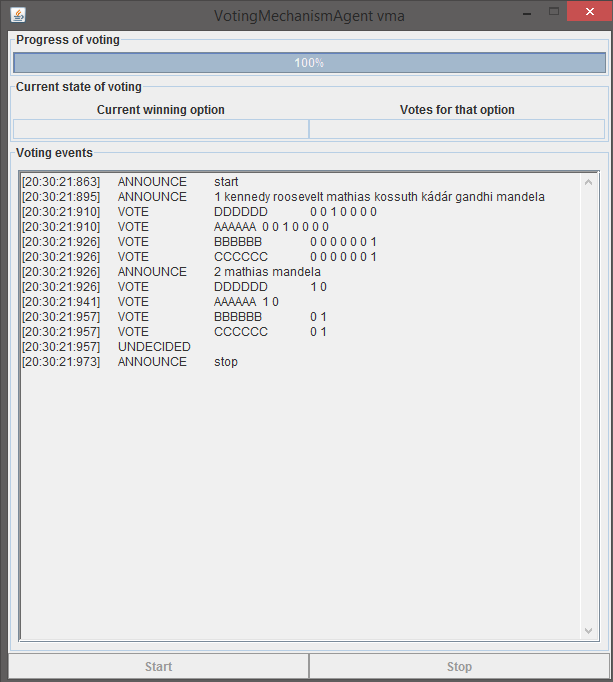
\includegraphics[height=7cm]{figures/ofel2.png}
\caption{Többfordulós szavazás}
\end{center}
\end{figure}

\section{Otthoni feladat 3}
\subsection{Leírás}
Alakítsa át a szavazást többségi elven működő szavazássá (majority rule voting)!
Ehhez  egészítse  ki  a  VotingMechanismAgent ágens  AnnounceAndWait
viselkedésének  action() metódusában, a  case 1 részben (mikor  state=1 , azaz az
ágens  szavazatokra  vár)  a  megfelelő  két  feltételvizsgálatot
( if(CommonMethods.maxNum(votes) == 1) ) úgy, hogy ne csak azt nézzék, hogy
egyetlen maximális minősítésű opció van-e az eddig beérkezett szavazatok alapján,
hanem azt is, hogy a szavazatok száma erre az opcióra legalább az ágensek számának
fele-e, vagy sem. Tesztelje a módosított szavazási protokollt az előbbi feladatokhoz
hasonlóan, és foglalja össze, ill. magyarázza meg a különbségeket és hasonlóságokat!
\subsection{Megoldás}

\begin{figure}[!h]
\begin{center}
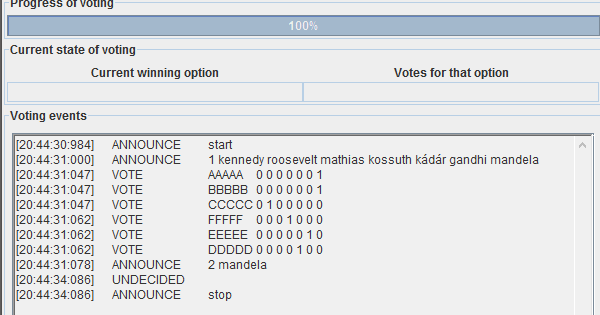
\includegraphics[height=7cm]{figures/ofel3_1.png}
\caption{Minősített többségi szavazás}
\end{center}
\end{figure}
\begin{figure}[!h]
\begin{center}
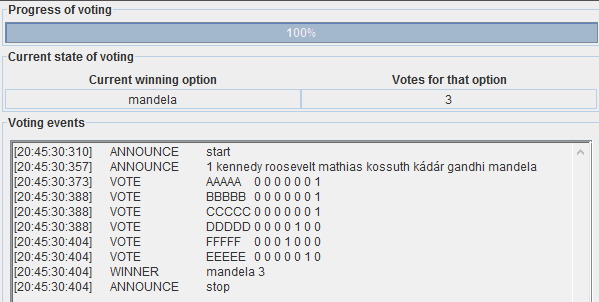
\includegraphics[height=7cm]{figures/ofel3_2.png}
\caption{Minősített többségi szavazás}
\end{center}
\end{figure}


\section{Otthoni feladat 4}
\subsection{Leírás}
Térjünk  most  át  az  aukciókra!  Indítson  el  legalább  három
msclab01.votingauction_lab.BidderAgent.BidderAgent licitáló ágenst (pl.  ba0 ,
ba1 , és  ba2 néven) a  auction01.cfg aukció
konfigurációval,  illetve  egy
msclab01.votingauction\_lab.AuctioneerAgent.AuctioneerAgent árverező
ágenst is (pl.  aa néven) ugyanezzel.
\begin{enumerate}
	\item Figyelje meg és értelmezze a működést.
	\item Kövesse nyomon Sniffer ágenssel az ágensek közti üzenetcserét.
	\item Mit tapasztal?
	\item Milyen szabályok szerint zajlik az aukció?
	\item Mi az előnye, és mi a hátulütője ennek a fajtájú aukciónak?
	\item A lefutás során/után milyen adatok jöttek létre a log
	könyvtárban?
	\item Milyen licitálási stratégia szerint játszik most a BidderAgent ágens?
	\item Szorgalmi feladat: próbáljon meg javítani a BidderAgent ágens licitálási stratégiáján, és
	magyarázza meg, hogy mit és miért csinált!
\end{enumerate}
\subsection{Megoldás}
\end{figure}
\begin{figure}[!h]
\begin{center}
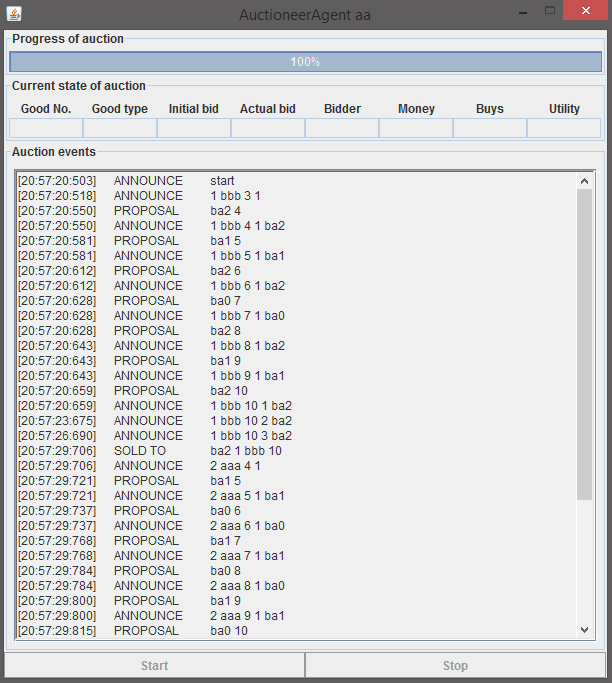
\includegraphics[height=7cm]{figures/ofel4.png}
\caption{Minősített többségi szavazás}
\end{center}
\end{figure}


\section{Labor feladat 1}
\subsection{Leírás}
Alakítsa át a VoterAgent szavazó ágenst úgy, hogy ne csak egy, hanem több opcióra is
képes legyen egy-egy körben szavazni (ehhez akár a VotingMechanismAgent ágens
szavazási konfigurációjához hasonló konfigurációt is létrehozhat számára, vagy átadhatja a
több óhajtott opciót bemeneti paraméterként, ha egyszerűbb, vagy lehet akár véletlenszerű is,
hogy mire szavaz az ágens)! Ehhez a ParticipateInVoting viselkedés case 1 esetét
kell módosítani. Ennek kapcsán ne felejtse el kivenni a VotingMechanismAgent ágens
AnnounceAndWait viselkedésének action() metódusában a case 1 rész for
ciklusából a break-et. Tesztelje a működést! Mit tapasztal? Hogyan zajlik ez az újfajta,
úgynevezett engedélyező szavazás (approval voting)? Mi a különbség, hasonlóság, előny,
hátrány az előzőleg megvalósított/kipróbált módszerekhez képest?
\subsection{Megoldás}

\section{Labor feladat 2}
\subsection{Leírás}
\subsection{Megoldás}

\section{Labor feladat 3}
\subsection{Leírás}
\subsection{Megoldás}

\section{Labor feladat 4}
\subsection{Leírás}
\subsection{Megoldás}


\section{Labor feladat 5}
\subsection{Leírás}
\subsection{Megoldás}

\section{Összefoglalás}
A labor során megismerkedtem a játékok GAMBIT-al való leírásával, megoldásával. Ez követően szimulációkat végeztem JADEX ágensekkel, akik lejátszották az adott játékokat. Tapasztaltam hogy a játékok világában a leírás exponenciálisan nő a játékosok, lehetséges lépések számával. Kis lépésszám melett a GAMBIT alkalmas volt a játék modellezésére, de nagy lépésszámnál a Nash egyensúly számolás és domináns stratégia keresés már sikertelen volt.